\section{Evaluation}
We evaluate scheduling overhead and qos management performances.

・優先度スケジューリングの評価はしなくてよいのか

・GPUSyncと比較しなくて良いのか

・実アプリで動かすとどうなるのか

本稿における評価では、本Linux-RTXGを利用した際のオーバヘッドを定量的に計測し、利用に伴ってどれだけのデメリットを含んでいるかを提示する。
定性的な評価としては関連する研究と保持する機能や特徴の差について次章でdiscussする。

\subsection{Experimental Environment}
Our experiments are conducted with the Linux kernel 3.16.0 on NVIDIA Geforce GTX680 graphics card and 3.40GHz Intel Core i7 2600, which contains 8 cores (including the two hyper-threading cores) and 8GB main memory.
GPU programs are written in CUDA and compiled by NVCC v6.0.1.
GPU drivers are used NVIDIA driver 331.62 and Nouveau driver linux-3.16.0.
CUDA libraries are used NVIDIA CUDA-6.0 and gdev.
%CPUはIntel Core i7 2600 3.40GHz、
%4GB*2のメモリ、GPUはGeForce GTX680を用いる。
%KernelはLinux kernel 3.16.0を用い、ディストリビューションはUbuntu 14.04である。
%CUDAコンパイラはNVCC v6.0.1、CUDAランタイムはcuda-6.0 or Gdev、GPUドライバはNVIDIA (331.62)、Nouveau (linux-3.16.0)を用いる。
%各ランタイム、ドライバは評価項目ごとに使い分ける。

\subsection{Interrupt intercept overhead}
まずInterrupt interceptのオーバヘッドの測定を行う。
本評価では、GPUドライバはnouveauを用いる。
割り込み処理は、各割り込みの種類によって、処理時間が異なり、その分布は一様ではないため、単に測定して平均をとっても比較ができない。
そのため各割り込みの種類の判別のためにNouveauを用いて、割り込みの種類が同一のもので、カーネル内のdo\_IRQ関数内でハンドラが呼ばれてから終了までの時間を測定し
どの程度のオーバヘッドで割り込みの盗聴及び、盗聴した割り込みがいずれのカーネルに関連したものであるかの識別ができるかどうかを測定する。

\begin{figure}[t]
\begin{center}
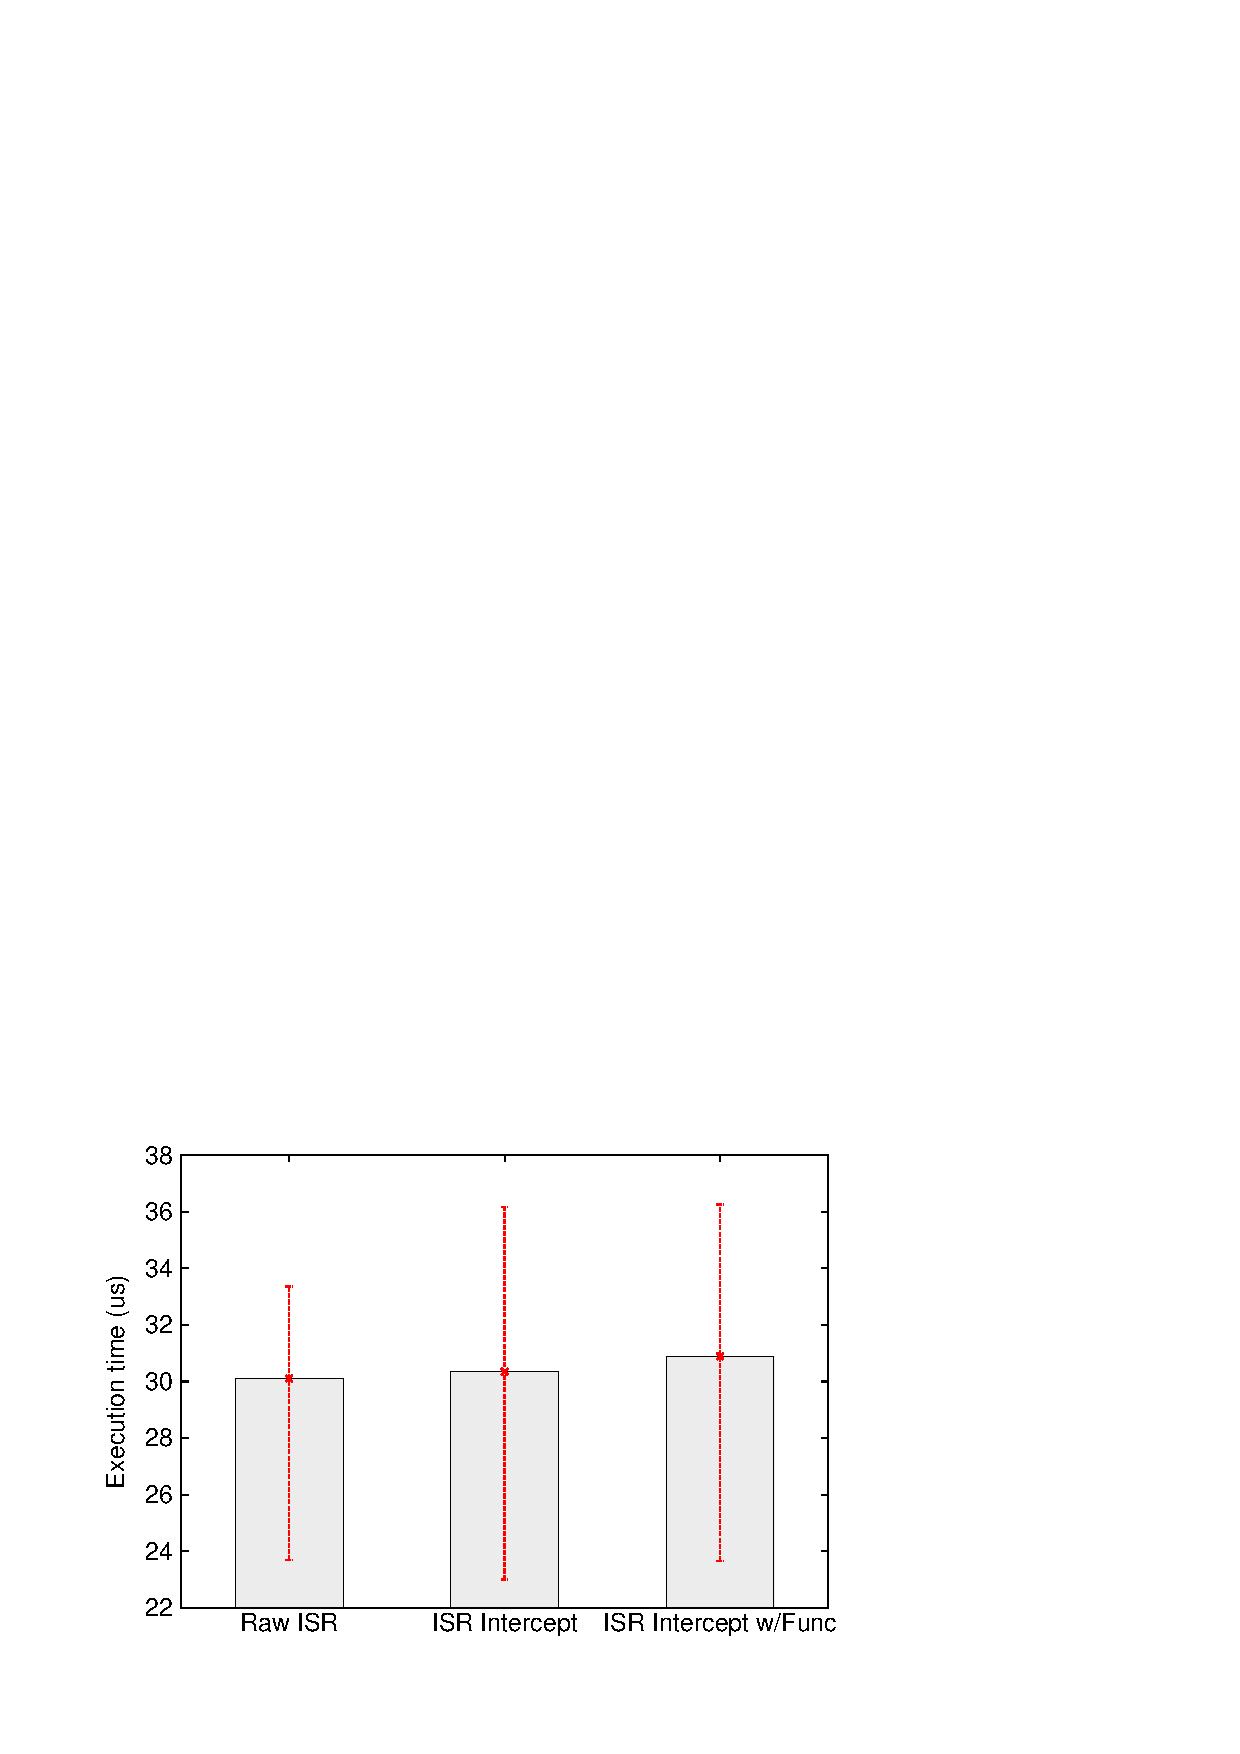
\includegraphics[width=0.4\textwidth]{img/interrupt.pdf}
\caption{Interrupt intercept overhead}
\end{center}
\label{fig:irq_overhead}
\end{figure}

Figure \ref{irq_overhead}は上記設定で測定した結果である。
Raw ISRは通常のルーチンで実行されるISR、ISR Interceptは割り込みを盗聴するのみ、
ISR intercept w/Funcは盗聴した上でその割り込みが、いずれのカーネルに関連した割込みか識別しスケジューラを立ち上げる機能を実行した場合である。
それぞれ1000回の測定で平均値を取り、最小値と最大値についてエラーバーで示している。
この図から見て取れるように、オーバヘッドは確実に存在する。
ISR Interceptだと247nsのオーバヘッドであり、
ISR Intercept w/Funcでも790nsのオーバヘッドである。
この数値は直感的に考えると小さくシステム自体に影響を及ぼすほどではないと考えられ、
しかしその割込みが乱発することによる積み重ねによっては影響を与えることは、
本手法のデメリットとして意識しなければならない。


\subsection{Independent generate sign for Synchronization overhead}
本稿では同期用サイン生成のためのオーバヘッドを測定する。
割込みの立ち上げは同期を求めるタイミング(e.g. カーネルラウンチ後)にrtx\_nvrm\_notify()を呼び出す必要がある。
スケジューリングを行わないVanillaな状態ではこれらのAPIは必要ではないものであるため、これらのAPIにかかった時間はすべてオーバヘッドとなる。

そのためこれらのオーバヘッドの計測を行う。
計測はAPIの呼び出しから戻るまでを測定する。

\begin{figure}[!t]
\begin{center}
\subfigure[Part of Initialize]{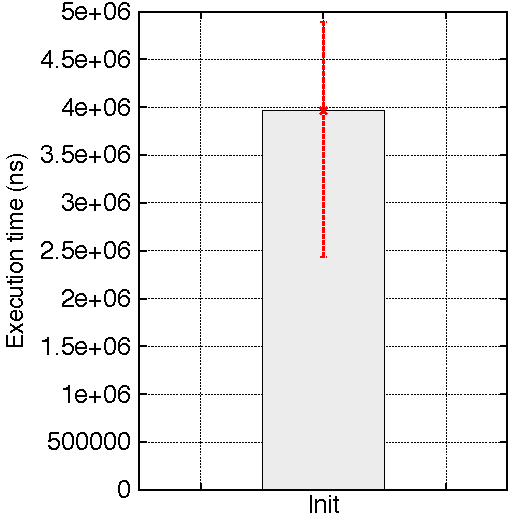
\includegraphics[width=0.23\textwidth]{img/irq_rise_init.pdf}}\subfigure[Part of notify]{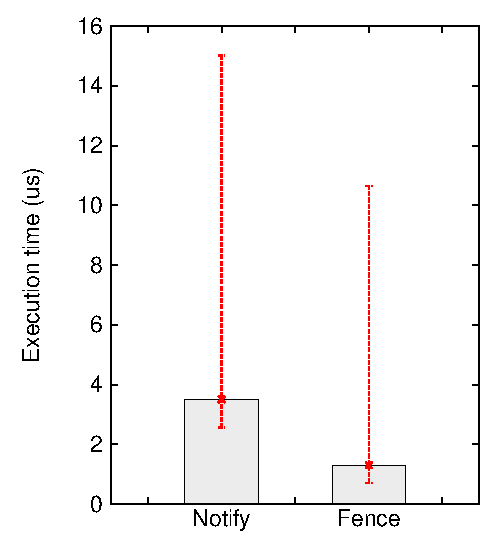
\includegraphics[width=0.23\textwidth]{img/irq_rise_notify.eps}}
\caption{Interrupt raised method overhead}
\label{fig:irq_rise_overhead}
\end{center}
\end{figure}

結果をFigure \ref{fig:irq_rise_overhead}に示す。
InitializeはIndirect Bufferはプロセスが立ち上がるたびに、
コマンド送信用のIndirect Bufferの確保や各エンジンの登録のために呼び出される必要がある。
Notifyはカーネル実行後や非同期メモリコピー実行後のような実際に割込みを発生させたいタイミングで呼び出される。
これらはioctlシステムコールによってユーザ空間とカーネル空間をまたいでる影響か、実行時間のバラ付きが大きく出ている。

Initializeは比較的時間がかかっているが、1プロセスにつき一度しか呼ばれないため、アプリケーション全体への影響は少ないと考えられる。
Notifyに関してはそれほど時間がかかっておらず、同期待ちの間に実行されるべき処理なため、こちらもアプリケーション全体への影響は少ないと考えられる。
FenceについてもNotifyと同様に平均で2000ns以下とほぼ誤差といってもよい程度の時間である。

\subsection{Scheduling Overhead}\label{sec:eval:sched_overhead}

rtxでスケジューリングした場合のオーバヘッドを測定するために、"vanilla", "mutex", "rtx"の3種類のアプリケーションを用意した。
全てに共通するのが、1個のアプリケーションに複数のタスクが存在しており、
各タスクには10個のジョブが含まれることである。1個のジョブはGPUへのデータ転送、GPUカーネル実行、GPUからのデータ転送を含んでいる。GPUカーネルは単純な行列の計算を行う。

3種で異なる点として、まずmutexは同時にlaunchが発行されるのが1つに調停されるようにmutexを用いてロックしたバージョンである。
そしてrtxはlinxu-rtxgを用いて実行したケースであり、
vanillaはそれらの追加が無くスケジューリングや調停を一切行わないケースである。

CPUのスケジューリングはlinux-rtxを用いたシンプルなFixed-priorityスケジューリング (LinuxのSCHED\_FIFOと同様のポリシー、ジョブ管理のみを行う)を用いる。
GPU側のスケジューリングは、Gdevで提案されたBANDスケジューラ、Linux-RTXでの同期は全てNOTIFYを用いて行う。

計測結果をFigure~\ref{fig:fp_overhead}に示す。
アプリケーションに含まれるタスク数ごとにプロットしており、各ジョブ内のラウンチ要求から実行完了までにかかった時間の平均値を各処理毎に積み上げ式で示している。


\begin{figure}[t]
\begin{center}
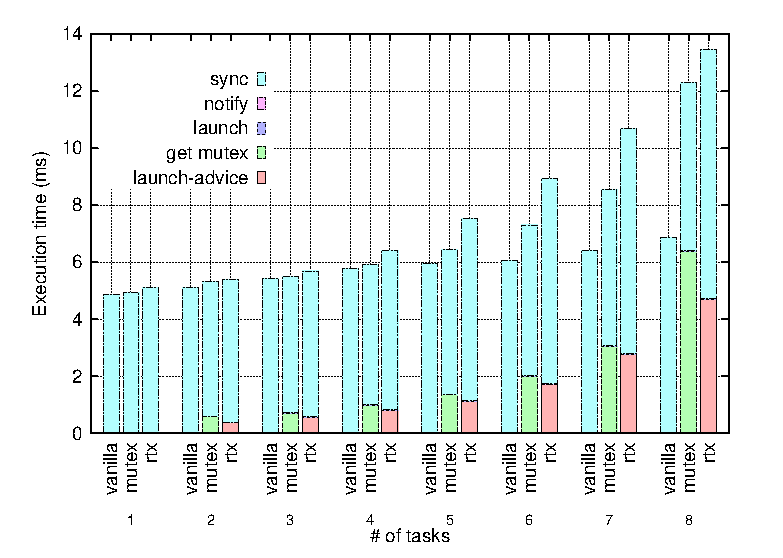
\includegraphics[width=0.5\textwidth]{img/sum_task_fp.eps}
\caption{Scheduling overhead(between GPU kernel launch request and synchronization)}
\end{center}
\label{fig:fp_overhead}
\end{figure}

\TODO{結果について説明と、考察}

launch\_adviceはrtx\_gpu\_launchによってGPU利用のためのリクエストを出してから、許可がでるまでを示しており、
get\_mutexはmutexによってロックを獲得するまでの時間、
launch、notifyはそれぞれコマンドを発行するまでにかかった時間で、
syncは発行されてから同期完了するまでの時間である。
全て、100回のアプリケーション実行($number of tasks ☓$)

\begin{figure}[t]
\begin{center}
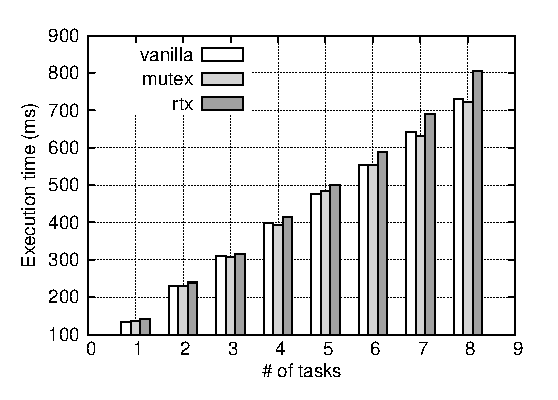
\includegraphics[width=0.5\textwidth]{img/sum_task.eps}
\caption{Scheduling overhead (Time of entire task)}
\end{center}
\label{fig:fp_overhead}
\end{figure}


\subsection{QoS Management}

次にGPUのバジェットエンフォースメントの性能を評価する。
ここでは、今回同一アルゴリズムでQoSマネージメントを行っているGdevとの比較を行い、
パッチを利用しない実装においても、性能をほぼ落とすこと無くできていることを示す。

比較対象は、本Linux-RTXGと同様のスケジューリングアルゴリズムが提供可能なGdevのモジュール版とで比較する。
評価に用いるスケジューリングポリシーはBANDスケジューラを用いる。
実験に利用するアプリケーションとして、\ref{sec:eval:sched_overhead}節で利用したものと同様のものでTaskを4つ生成し、各タスク毎に25\%のGPU利用権限を与える。
これらのタスクの実行中のGPU利用率を計測し、Gdevと同様のアルゴリズムを用いることで、今回提供するLinux−RTXGによるアプローチによってどれだけQoSマネージメントについてのパフォーマンスに影響するかを示す。
Gdevを用いることから、両者ともデバイスドライバはNouveauドライバを用いる.


\begin{figure}[t]
\begin{center}
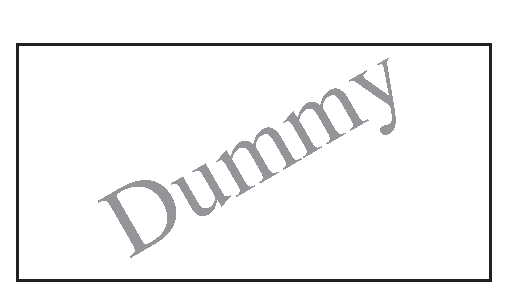
\includegraphics[width=0.5\textwidth]{img/dummy}
\caption{Utilization of four tasks on the Linux-RTXG only priority scheduling. Each tasks are given different priorities.}
\end{center}
\label{fig:qos_rtx}
\end{figure}

\begin{figure}[t]
\begin{center}
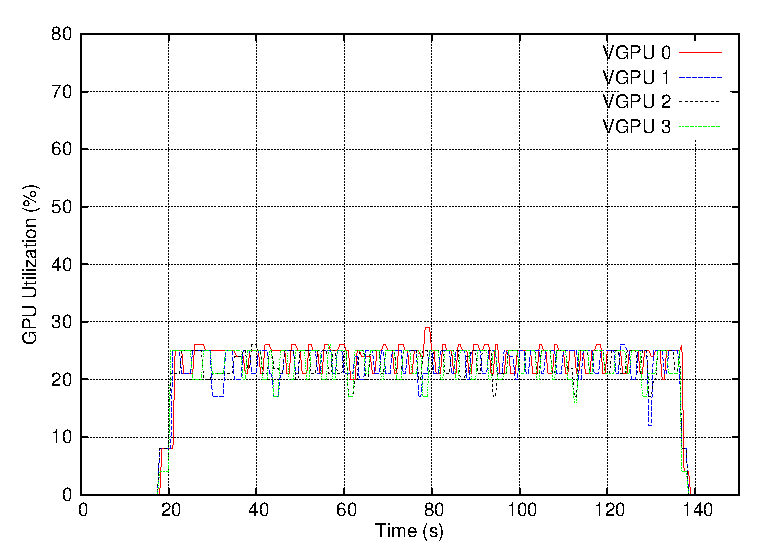
\includegraphics[width=0.5\textwidth]{img/rtx_qos.eps}
\caption{Utilization of four tasks on the Linux-RTXG resource reservation. Each tasks are given different priorities and all tasks are fairly given resources which is 25\%}
\end{center}
\label{fig:qos_rtx}
\end{figure}

\begin{figure}[t]
\begin{center}
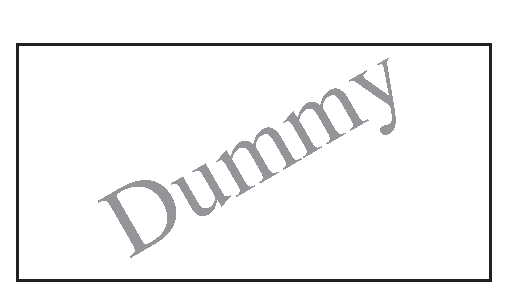
\includegraphics[width=0.5\textwidth]{img/dummy}
\caption{Utilization of four tasks on the Gdev resource resevation. All tasks are fairy given resources which is 25\%}
\end{center}
\label{fig:qos_gdev}
\end{figure}

Figure~\ref{fig:qos_gdev},\ref{fig:qos_rtx} show gpu usage on the qos management by gdev and linux-rtxg.
\TODO{結果に合わせて記述}


%%%

Figure~\ref{} shows 
